\chapter{Data integrity}
\label{cha:state_of_the_art}
High-quality data availability and integrity property is a must-have
requirement in many IT systems. A lot of enterprise and scientific effort
has been put into development of tools and methods that support this capability.
From cryptographic hash-based mechanisms that enable corruption discovery, to
replication and error-correcting codes for data recovery, to security
mechanisms preventing malicious data corruption. However, emerging trends in IT
solutions, as cloud computing, put new challenges in this area. The following
chapter presents the state of the art.\\

This chapter presents an introduction to a~set of topics connected with 
data integrity in cloud storage. In the first section we present
general methods and tools for ensuring data integrity which form
fundamanetal building blocks for more advanced methods. Further, we
describe cloud storage model, we focus on its origins and advantages, but
also discuss limitations of its interface and SLA contracts. In the last
section we dive into the subject of assuring data integrity in cloud
storage and present some emerging methods: proofs of retrievability (PORs)
and data integrity proofs (DIPs).



	\section{General methods and tools for ensuring data integrity}
	\label{classic-integrity-methods}
Providing a way to check the integrity of information transmitted over or
stored in an unreliable medium is a prime necessity in the world of open
computing and communications. The following section presents security building
blocks that enable data integrity assurance. The cryptographic hash functions
are core components of message authentication code algorithm to provide message
integrity and authenticate the message creator. Error correcting codes are 
commonly deployed to be able to retrieve the original data after partial
corruption.
 
		\subsection{Cryptographic hash functions}
A cryptographic hash function is a hash algorithm that maps a message of
arbitrary length to a fixed-length message digest (hash value). These
algorithms enable determination of a message's integrity: any change to the
message will, with high probability, result in a different message digest.
This property appears very useful as a building block in various security
constructions from generation and verification of digital signatures, to
message authentication codes, to generation of random numbers.\\ 

A cryptographic hash function is expected to have the following properties
\cite{nist-hash}:\\

\begin{itemize}
	\item \textbf{Collision resistance}: that it is computationally infeasible
	to find two different hash function inputs that have the same hash value.
	In other words, it is computationally infeasible to find $x$ and $x'$ for
	which $hash(x) = hash(x')$.
	\item \textbf{Preimage resistance}: that given a randomly chosen hash
	value, $hash\_value$, it is computationally infeasible to find an x so that
	$hash(x) = hash\_value$. This property is also called one-way property.
	\item \textbf{Second preimage resistance}: that it is computationally
	infeasible to find a second input that has the same hash value as any other
	specified input. That is, given an input $x$, it is computationally
	infeasible to find a second input $x'$ that is different from $x$, such
	that $hash(x) = hash(x')$.
\end{itemize}

Currently, the Secure Hash Standard (SHS) \cite{fips-shs} specifies five
approved hash algorithms: SHA-1, SHA-224, SHA-256, SHA-384 and SHA-512. Their
strengths of the security properties discussed above, vary significantly. While
one cryptographic hash function is suitable for one application, it might not
be suitable for other. The general trend is that the longer the message digest
(its hash), the stronger security guarantees, but also higher computational
complexity.\\

Additionally, the algorithms differ in terms of the size of the blocks and
words of data that are used during hashing or message digest sizes. They are
presented in table \ref{tab:hash-comparison}.

\begin{table}[h!]
\centering
\begin{tabular}{|l||c|c|c|c|}
	\hline
	Algorithm & Message Size (bits) & Block Size (bits) & Word Size (bits) & Message Digest Size (bits) \\ \hline \hline
	SHA-1   &  $< 2^{64}$ &  512 & 32 & 160 \\ \hline
	SHA-224 &  $< 2^{64}$ &  512 & 32 & 224 \\ \hline
	SHA-256 &  $< 2^{64}$ &  512 & 32 & 256 \\ \hline
	SHA-384 & $< 2^{128}$ & 1024 & 64 & 384 \\ \hline
	SHA-512 & $< 2^{128}$ & 1024 & 64 & 512 \\ \hline
\end{tabular}
\caption{Secure hash algorithm properties \cite{fips-shs}}
\label{tab:hash-comparison}
\end{table}

		\subsection{Error correcting codes}
An error-correcting code (ECC) is an algorithm for expressing a sequence of
numbers such that any errors which are introduced can be detected and corrected
(up to certain level) based on the remaining numbers. All error
correcting codes are based on the same basic principle: redundancy is added to
information in order to correct any errors that may occur in the process of
storage or transmission. In practice, the redundant symbols are appended to the
information symbols to obtain a coded sequence (codeword).\\

ECC can be divided into two classes:\\

\begin{itemize}
	\item \textbf{block codes}: that work on fixed-size blocks of predetermined
	size,
	\item \textbf{convolutional codes}: that work on bit streams of arbitrary
	length.
\end{itemize}

Among classical block codes the most popular are Reed-Solomon codes which are
in widespread use on the CDs, DVDs and hard disk drives. Hamming codes are
commonly used to prevent NAND flash memories errors. On the other hand,
convolutional codes are widely used in reliable data transfer such as digital
video, radio, mobile and satellite communication. Both block and convolutional
codes are often implemented in concatenation.\\

Apart from embedding ECC in the hardware solutions, they are also being applied
in software constructions to recover from eventual data corruption.

		\subsection{Message authentication codes}
A message authentication code (MAC) is an authentication tag (also called 
a~checksum) derived by applying an authentication scheme, together with 
a~secret key, to a message \cite{nist-hmac}. The purpose of a MAC is to
authenticate both the source of a message and its integrity without the use of
any additional mechanisms.\\

MACs based on cryptographic hash functions are known as HMACs. They have two
functionally distinct parameters: a message input and a secret key known only
to the message originator and intended receivers.\\

An HMAC function is used by the message sender to produce a value (the MAC)
that is formed by condensing the secret key and the message input. The MAC is
typically sent to the message receiver along with the message. The receiver
computes the MAC on the received message using the same key and HMAC function
as were used by the sender, and compares the result computed with the received
MAC. If the two values match, the message has been correctly received, and the
receiver is assured that the sender is a member of the community of users that
share the key \cite{nist-hmac}.\\

To compute a MAC over the data $text$ using the HMAC function with key $K$, the
following operation is performed \cite{nist-hmac}:

\begin{equation}
	MAC(text) = HMAC(K, text) = H(((K_{0} \oplus opad)||H((K_{0} \oplus ipad) || text)))
\end{equation}

where:

\begin{itemize}
	\item \textbf{$K_{0}$} -- the key $K$ after any necessary pre-processing to
	form a $B$ byte key,
	\item \textbf{$ipad$} -- inner pad, the byte $0x36$ repeated $B$ times,
	\item \textbf{$opad$} -- outer pad, the byte $0x5c$ repeated $B$ times,
	\item \textbf{$B$} -- block size (in bytes) of the input to the $H$ hash function,
	\item \textbf{$H$} -- an approved hash function.
\end{itemize}

The Internet Engineering Task Force (IETF) published a RFC document to describe
HMAC \cite{rfc2104}.\\

Apart from HMAC, a couple of other MACs have been proposed. Stinson
\cite{unconditional-mac} presented an unconditionally secure MAC based on 
encryption with a one-time pad. The cipher text of the message authenticates
itself as nobody else has access to the one-time pad. Lai et al.
\cite{stream-mac} proposed a MAC based on stream ciphers. In their algorithm,
a~provably secure stream cipher is used to split a message into two substreams
and each substream is fed into a linear feedback shift register (LFSR); the
checksum is the final state of the two LFSRs.\\

	\section{Cloud storage model}
	\label{cloud-model}
Cloud computing is an emerging IT trend toward loosely coupled networking of
computing resources. Its core feature is to move computing and data away from
desktop and portable PCs to large data centers and provide it as a service. The
popularity of this paradigm develops as it reduces IT expenses and provide
agile IT services to both, organisations and individuals. Additionally, users
are released from the burden of frequent hardware updates and costly
maintenance, while paying for cloud services on consumption basis.\\

While cloud computing represents the full spectrum of computing resources, this
work focuses on cloud storage services for archival and backup data. As it will
be shown, this technology, apart from its advantages, introduces many problems,
especially for ensuring data availability and integrity which may appear as
untrustworthy.   
		\subsection{General features}
Cloud storage is a model of broadband network access to virtualized pool of
storage resources on demand. In the spirit of cloud computing paradigm, it is 
mostly provided via REST/SOAP web service interface, however, other standard
protocols are used. Despite incompatibilities among various cloud storage
providers, as cloud computing gets more mature technology, their
interfaces begin to standardize. Storage Networking Industry Association (SNIA)
works toward developing a reference Cloud Data Management Interface (CMDI).\\

While different cloud storage solutions vary significantly, the following
common properties can be derived:

\begin{itemize}
	\item storage space is made up of many distributed resources, but still
	acts as one, virtualized layer,
	\item high fault-tolerance through redundancy and distribution of data,
	\item high data durability via object versioning,
	\item predominantly eventual consistency with regard to data replicas.
\end{itemize} 

Typically, public cloud providers expose storage space as object data store,
where data is organized into containers (or buckets). Each container consists
of data objects (files) on which standard create, read, update, delete (CRUD)
operations may be performed. Additional metadata is appended to containers and
data objects such as name, size, creation/modification date or hash checksum.\\

Amazon Simple Storage Service (S3) \cite{amazon-s3}, 
Rackspace Cloud Files \cite{rackspace-cloud} and
Google Cloud Storage \cite{google-cloud} are the most popular representatives
of the illustrated cloud storage model. Despite the increasing popularity of
public cloud storage providers, hybrid and private cloud solutions do exist,
Openstack Swift \cite{openstack-cloud} and 
Eucalyptus Cloud \cite{eucalyptus-cloud} to name just a few.\\

		\subsection{Interface and API}
Current cloud storage systems mostly provide REST/SOAP web service interface to
access the resources, in the spirit of Service Oriented Architecture (SOA)
paradigm. While this thesis focuses on this method of access and its
consequences, other providers expose different types of interface. Some of
them are presented in figure \ref{fig:cloud-access} with concrete examples of
solutions \cite{cloud-storage-anatomy}.

\begin{figure}[h!]
	\centering
	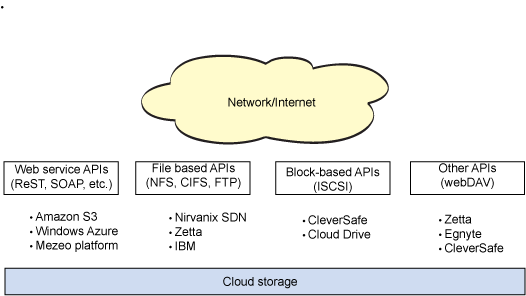
\includegraphics[width=0.8\textwidth]{images/cloud-access.png}
	\caption{Cloud storage access methods \cite{cloud-storage-anatomy}:
	major cloud storage providers focus on web service based access methods
	(SOAP and REST), however other solutions provide file-based, block-based
	or WebDAV forms of access.}
	\label{fig:cloud-access}
\end{figure}

Despite the fact that web service interfaces enable loose coupling and
technology interoperability, they require integration code with an application.
Many multi-cloud libraries were created to enable interoperability across
similar cloud services on a higher level of abstraction 
\cite{cloud-federation}. Their goal is to establish basic and uniform cloud
storage access layer at the API level \cite{jclouds, libcloud}.\\

Typically, cloud storage interfaces provide API to query, access and manage
stored data, which can be divided into the following groups
\cite{amazon-s3, rackspace-cloud, google-cloud, openstack-cloud, 
eucalyptus-cloud}:\\

\begin{itemize}
	\item \textbf{Operations for authentication}: to secure the access to
	cloud storage data (mostly via token-based authentication),  
	\item \textbf{Operations on the account}: to operate on account metadata
	such as managing existing containers and additional provider-specific data
	services,
	\item \textbf{Operations on the container}: to manage container policy, 
	versioning, ACLs, lifecycle and location,
	\item \textbf{Operations on the data objects}: to enable CRUD operations.
\end{itemize} 

There exists a growing trend to adjust provider-specific interfaces with the
SNIA reference model \cite{amazon-s3, rackspace-cloud, openstack-cloud}.
		
		\subsection{Service Level Agreement}
To provide high quality of service, cloud storage providers widely guarantee
Service Level Agreement (SLA) contracts. These are mostly related to service
availability during the billing cycle. The service downtime is considered as
cloud network error or response errors to a valid user requests. Currently,
most of the providers guarantee the availability level of $99.9\%$ of the time
\cite{amazon-s3, rackspace-cloud, google-cloud}.\\

However, if the provider will fail to provide a guaranteed level of service,
the appriopriate percentage of the credit is returned to the client. In this
sense, cloud storage should be still treated as best-effort. IT systems that
demand uninterrupted operation simply cannot entirely rely on it.\\

Moreover, eventual consistency model is inherently embedded into the
overwhelming majority of cloud storage architectures, which places new problems
to the solutions, where strict data consistency is a crucial requirement
\cite{metastorage, cloud-federation}. Besides eventual consistency, SLA
contracts still only address the service availability, while omitting data
integrity or retrievability speed issues. Even though, cloud storage service
with described limitations still fit to the vast number of market 
applications.\\

Customers who require a higher data availability and integrity guarantees,
still need to seek for hybrid solutions and develop sophisticated layers on
top of existing infrastructure to meet their demands.

		\subsection{Constraints and limitations}
Cloud storage architecture presented in previous section exhibit many
advantages to potential users. Nevertheless, it also introduces a couple of
drawbacks for demanding solutions.\\

The most striking consequence of cloud storage, is that data is stored remotely
on provider's resources and user has very limited possibilities to monitor or
check its data through abstract access layer. Even small security vulnerability
may compromise the data of all users in public cloud model.\\

As it was shown in previous subsection, cloud SLA contracts still lack strong
availability and integrity guarantees, rather than cost-return policy. Even
though cloud storage is perceived as superb technology, a couple of serious
downtimes have been reported in the last years. Amazon S3 users experienced
several unavailability and data corruption periods \cite{amazon-downtimes},
while Google Gmail lost data of thousands of accounts \cite{gmail-downtime} and
Google Docs enabled unauthorized access to the stored documents 
\cite{docs-downtime}.\\

Cloud storage REST/SOAP interfaces are flexible and rich in capabilities, but
when accessed remotely outside of cloud compute resources, they suffer from
network latency for each HTTP request. Downloading a fragment of a file pose
another challenge. It is mostly achieved by setting HTTP Range parameter to the
desired value. However, only single range value is permitted. It is particularly
problematic for data integrity monitoring protocols (presented in the next
section) as they request a lot of small file's blocks, and for each block 
a~separate HTTP request has to be sent, which means increased network
overhead.\\

Moreover, cloud storage solutions lack user's code execution capability over
stored data. The data has to be downloaded in order to perform computation. It
makes present data integrity monitoring protocols impractical and inefficient,
because they assume computation capability on the prover's side.

\section{Approaches to data integrity in cloud storage}
\label{cloud-integrity-approaches}
One of the fundamental goals of cryptography is data integrity protection.
Primitives such as digital signatures and message-authentication codes (MACs),
described in section \ref{classic-integrity-methods}, were created to allow
an entity in possession of a file $F$ to verify that it has not been tampered
with. The simplest way is to use keyed hash function $h_{k}(F)$ to compute and
store a hash value along with secret, random key $k$ prior to archiving a file.
To verify that the prover (remote server, cloud provider) possess $F$, the
verifier releases key $k$ and asks the prover to compute and return $h_{k}(F)$.
By using multiple keys with their corresponding hash values, the verifier can
perform multiple, independent checks. However, this approach introduces high
resource overhead. It requires the verifier to store large number
of hash values and the prover to read the entire file for every proof.\\

A more challenging problem is to enable verification of the integrity of $F$
without knowledge of the entire file's contents. It was firstly described in
general view by Blum et al. \cite{memory-correctness}, who presented efficient
methods for checking the correctness of program's memory. Following works
concerned dynamic memory-checking in a range of settings. For instance, Clarke
et al. \cite{clarke} consider the case of checking the integrity of operations
performed on an arbitrarily-large amount of untrusted data, when using only 
a~small fixed-sized trusted state. Their construction employ an adaptive
Merkle hash-tree over the contents of this memory. However, Naor and Rothblum
showed that online memory checking may be prohibitively expensive for many
applications \cite{omc-complexity}. This implies that applications requiring
memory checking should make cryptographic assumptions, or use an offline
version of the problem.\\

Unauthorized modifications to portions of files can be detected by
cryptographic integrity assurance upon their retrieval. But in its basic form
it does not enable such detection capability prior to the retrieval, what many
other schemes aim to provide.\\

One of the mostly developed model of ensuring integrity of remotely stored data
is the proofs of retrievability (POR). The first formal description of POR
protocol was proposed by Juels and Kaliski \cite{por}. In their scheme,
the client applies error-correcting code and spot-checking to ensure both
possession and retrievability of files. Shaham et al. \cite{compact-por}
achieve POR scheme with full proofs of security and lower communication
overhead. Bowers et al. \cite{por2} simplify and improve the framework and
achieve lower storage overhead as well as higher error tolerance. Later on, 
they extend it to distributed systems \cite{hail}. However, all these schemes
are focusing on static data. Before outsourcing the data file $F$ 
a~preprocessing steps are applied. Every change to the contents of $F$ require
re-processing, which introduces significant computation and communication
complexity. Stefanov et al. \cite{iris} propose an authenticated file-system
for outsourcing enterprise data to the untrusted cloud service providers with
the first efficient dynamic POR.\\

Atenise et al. \cite{pdp} presented the provable data possession (PDP) model
in order to verify if an untrusted server stores a client's data without file
retrieval. Key components of their scheme are public key based homomorphic
verifiable tags. In the subsequent work, Atenise et al. \cite{pdp2} described
a PDP scheme that uses only symmetric key cryptography. As a result, they
achieved lower performance overhead.\\

A couple of practical implementations for remote integrity assurance have been
developed. Bowers et al. \cite{hail} designed HAIL (High Availability and
Integrity Layer) which takes advantage of data distribution over a set of
servers to achieve efficient POR-like scheme. Shraer et al. \cite{venus}
created Venus, a scheme that guarantees integrity and consistency for a group
of clients accessing a remote storage provider. Venus ensures that each data
object read by any client has previously been written by some client.
Additionally, it protects against retrieving older version of the object.
Bessani et al. \cite{depsky} implemented DEPSKY, a system that improves the
availability, integrity and confidentiality of information stored in the cloud
through encryption, encoding, and replication of data on diverse clouds that
form cloud-of-clouds.\\

In the following subsections we examine exhaustively a couple of schemes
mentioned above. We present their architecture, advantages and limitations.

\subsection{Proofs of retrievability}
In a POR \cite{por, por2} protocol, a file is encoded by a client before
deploying it on cloud storage for archiving. Then, it employs
bandwidth-efficient challenge-response scheme to probabilistically guarantee
that a file is available at remote storage provider. Most of POR protocols 
proposed to date, use the technique of spot-checking in the challenge-response
protocol to detect data corruption. In each challenge, a subset of file blocks
is verified, and the results of a computation over these blocks is returned to
the client. The returned results are checked using the original checksums
embedded into the file at encoding time.\\

The primary POR-like protocol we consider in detail, was proposed by Juels and
Kaliski \cite{por} -- a MAC-based POR scheme. In this approach, they firstly
preprocess the file $F$ by applying error-correcting codes and MAC checksums
in the following steps:

\begin{enumerate}
	\item \textbf{Error correction}: the file is divided into $b$ blocks of the
	same length and apply an $(n,k,d)$-error correcting code,
	which expands each chunk of size $k$ into size $n$ and is able to recover
	from up to $d-1$ errors. The resulting file is denoted as $F'$.
	\item \textbf{Encryption}: the file with appended ECCs is encrypted.
	\item \textbf{MAC computation}: a $m$ number of blocks are selected in
	$F''$, their MACs computed and appended to the file.
	\item \textbf{Permutation}: of file blocks to secure appended MACs against
	corruption.
\end{enumerate}

The graphical presentation of the process is depicted in figure \ref{fig:por-modified-file}.\\

\begin{figure}[h!]
	\centering
	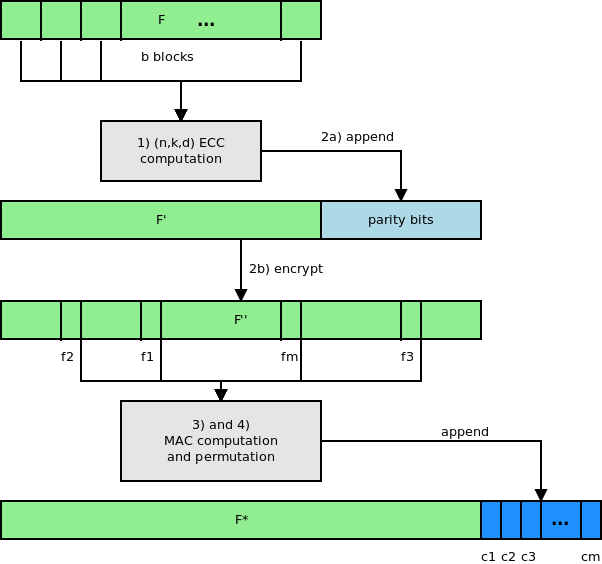
\includegraphics[width=0.8\textwidth]{images/por-schematic.png}
	\caption{Schematic presents POR based file encoding. Firstly (1), the file is divided into
	$b$ blocks and error correcting codes are applied to each of the block. Then (2), the
	parity bits are appended and the resulting file is encrypted. Finally (3,4), $m$ blocks of the encrypted
	file are selected, their MACs computed and appended to the file in permuted sequence. The resulting
	file is stored in archive \cite{por}.}
	\label{fig:por-modified-file}
\end{figure}

In the same paper \cite{por}, Juels and Kaliski proposed a sentinel-based POR
scheme. Similarily to the MAC-based approach it utilizes ECCs, but rather than
chosing MAC blocks it embeds sentinels in random positions in $F$, sentinels
being randomly constructed values. It is important that sentinels shall be 
indistinguishable from the encrypted file contents. The scheme consists of the
following steps:

\begin{enumerate}
	\item \textbf{Error correction}: the file is divided into $b$ blocks of the
	same length and apply an $(n,k,d)$-error correcting code,
	which expands each chunk of size $k$ into size $n$ and is able to recover
	from up to $d-1$ errors. The resulting file is denoted as $F'$.
	\item \textbf{Encryption}: the file with appended ECCs is encrypted.
	\item \textbf{Sentinel creation}: the randomly constructed sentinels are
	embedded in random positions in $F'$
	\item \textbf{Permutation}: which randomizes sentinel positions.
\end{enumerate}

In both approaches, if the prover has modified or deleted a substantial 
$e$-portion of $F$, then with high probability, also change roughly an
$e$-fraction of MAC-blocks or sentinels, respectively. It is therefore unlikely
to respond correctly to the verifier. Upon file retrieval, the user verifies
file's checksum. If it is not valid, then it starts file recovery based on
stored ECCs.\\

Of course, application of an error-correcting (or erasure) code and insertion
of sentinels enlarges $F^{*}$ beyond the original size of the file F. The
expansion induced by both POR protocols, however, can be restricted to a modest
percentage of the size of F. Importantly, the communication and computational
costs of the protocols are low.\\

The obvious advantage of the presented schemes is that they can be
parameterized.\\

Subsequent POR works \cite{compact-por, por2, hail, venus, iris} introduced
further optimizations to the solution described. The most important are:
moving MAC computation to the prover side and precomputing partial checksum
values.\\

However, POR-like schemes are not free from drawbacks. The primary limitation
is that preprocessing phase introduces non-negligible computational overhead.
Moreover, it requires storage of file $F$ in modified form. What is even more
problematic, it assumes that storage service provides user's code execution
capability, which is not true for current cloud storages 
(see section \ref{cloud-model}). For this reason, practical POR-like
implementation would require moving prover logic for computing 
challenge-response queries to the verifier. As a consequence, each access to
the portion of a file (MAC block or sentinel) would require separate HTTP
request. As many such accesses are performed per each file, it would be
impractical (except for large files, for which hundreds of short HTTP requests
would be faster than downloading the entire file).

\subsection{Data integrity proofs}
Data integrity proof (DIP) \cite{dip} is a protocol, which just like POR, aims
to assure that the remote archive poses the data. Unlike POR schemes, it does
not involve any modifications to the stored file. The client before storing
data file $F$, preprocesses it to create suitable metadata, which is used in
the later stage of data integrity verification. The preprocessing stage
consists of the following steps:

\begin{itemize}
	\item \textbf{Generation of metadata}: the file $F$ in divided into $n$
	blocks that each are $m$ bits length. Then, for each data block, a set of
	$k$ out of $m$ bits are selected. The value of $k$ is in the choice of the
	verifier and is a secret known only to him. Therefore, we get $n*k$ bits in
	total.
	\item \textbf{Encrypting the metadata}: each of the metadata from the data
	blocks, is encrypted by using a suitable algorithm and concatenated.
	\item \textbf{Appending the metadata}: all the metadata are appended to the
	file $F$, however, they can be also stored in the verifier.
\end{itemize}

The graphical presentation of the process is depicted in figure \ref{fig:dip-schematic}.\\

\begin{figure}[h!]
	\centering
	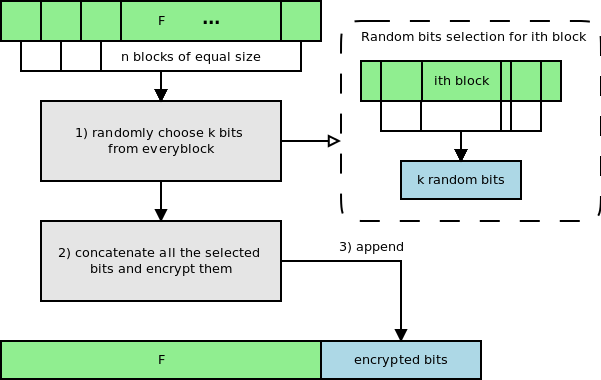
\includegraphics[width=0.8\textwidth]{images/dip-schematic.png}
	\caption{Schematic presents DIP based file encoding. Firstly (1), the file is
	divided into $n$ blocks of equal size and $k$ randomly chosen bits are selected
	out of each block. Then (2), concatenated bits from all of the blocks are encrypted
	and appended to the file $F$ \cite{dip}.}
	\label{fig:dip-schematic}
\end{figure}

To verify $F$ integrity, the verifier utilizes challenge-response mechanism. In
each challenge, it verifies a~single block $i$ specifing the positions of the
$k$ selected bits and retrieves encrypted metadata for this block to compare
the values. Any mismatch between the two would mean a loss of the integrity of
the clients data at the cloud storage.\\

While DIP scheme seems trivial, it eliminates a couple of disadvantages of the
POR approach. Firstly, data integrity assurance does not require any
modifications to the stored file, but also prevents the data recovery
capability by ECC. It also exhibits negligible computational overhead.
However, it still either assumes user's code execution capability by cloud
provider or requires large number of accesses to non-continuous data fragments.
Such data acceses are performed in separate HTTP requests in the current
cloud storages (see section \ref{cloud-model}), which is practically
infeasible.\\ 

\section{Summary}
In this chapter an important topics regarding data integrity and cloud storage were presented.
General methods and tools for ensuring data integrity such as cryptographic hash functions,
error correcting codes and message authentication codes were discussed. They form a set of
fundamental building blocks and patterns used in more advanced methods. Its understanding 
is crucial in further discussion on data integrity throughout this thesis. Further, the
overview of cloud storage model was presented. We focused on describing its origins in connection
with advantages which it brings in numerous applications. The discussion also includes the
high-level description of cloud storage interface and SLA contracts. We also stress the contraints
and limitations of moving the data to the cloud. Shortly, recent cloud providers failure reports
and the best-effort SLA contracts question the applicability of cloud storage in areas
such as medical care and flight services. In the last section, we extensively discuss current
approaches to data integrity in the cloud. We mainly focused on two developing schemes: proofs
of retrievability (PORs) and data integrity proofs (DIPs), but also mention other solutions and
improvements. 
